\newpage
\section{Обзор предметной области}
\label{review}

\subsection{Методы машинного обучения} 
\label{ML}
В разделе \ref{MLINTRO} было приведено неформальное введение в теорию машинного обучения. В данном приведена более формальная постановка задачи машинного обучения и описан один из наиболее используемых методов ее решения - метод опорных векторов, котороый, как показано в \cite{ROZ}  может быть успешно применен к задаче фильтрации спама. 
\subsubsection{Обучение по прецедентам}
Сформулируем основную задачу машинного обучения.

\textit{
Пусть есть неизвестная функция $F: X \rightarrow Y$, переводящая объекты
множества $X$ в объекты множества $Y$, причем для некторых $x_1, x_2, ... x_n$ известны соответсвующие им значения $y_1 = F(x_1), y_2 = F(x_2), ... y_n = F(x_n)$.
Необходимо построить функцию $F^*(X)$, наилучшим образом приближающую $F(X)$.
}

Под фразой \textbf{наилучшим образом приближает} подразумевается, что для некоторого функционала качества $\mu(y, y')$, матожидание
\begin{equation}
\label{matozh}
E\mu(F(x), F^*(x)), x \in X
\end{equation}
будет минимальным.

В качестве $\mu(y, y')$ можно брать например модуль разности, квадрат разности и т. п.

Объект $x_i$ для которого известно соответсвующее значение $y_i$ называется \textbf{прецедентом}

\textbf{Методом обучения} называется проецесс построения $F^*(x)$ по парам $(x_1, y_1), (x_2, y_2), ... (x_n, y_n)$. Множество таких пар называется \textbf{обучающей выборкой}

Построенную функцию $F^*(x)$ часто также называют \textbf{алгоритмом}, подразумевая,  что она должна быть эффективно вычислима на компьютере.

Задача построения такого алгоритма в общем случае не может быть решена точно, так как неизвестна природа исходной функции $F(x)$. Кроме того минимизация $\mu$ на обучающей выборке не обязательно приводит к тому, что и на новых объектах из $X$ значение $\mu$ также будет мало(см. раздел \ref{overfitting}).
%TODO смотри пример(рисунок, переобучение)

Процесс построения модели можно также рассматривать как выбор конкретного значения функции $F^*(x)$ из семейства $F^*(x, \pi)$. Значение выбранного параметра $\pi$ в таком случае называется \textbf{моделью} для алгоритма
$F^*(x)$

В целом процесс решения задачи машинного обучения называют \textbf{машинным обучением} или \textbf{обучением по прецедентам}

Если множество $Y$ конечно, то говорят, что поставленная задача  является \textbf{задачей классификации} с $m$ классами, где $m$ - мощность множества $Y$.

Задачу классификации можно также поставить вероятностно:

\textit {
Пусть есть неизвестная функция $F: X \rightarrow Y$, переводящая объекты
множества $X$ в объекты множества $Y$, причем множество $Y$ конечно. Пусть также для некторых $x_1, x_2, ... x_n$ известны соответсвующие им значения $y_1 = F(x_1), y_2 = F(x_2), ... y_n = F(x_n)$ Необходимо построить фукцию $F^*(x, y): (X, Y) \rightarrow [0, 1]$, возвращающую оценку вероятности того, что $F(x)=y$
}

Задача фильтрации спама по своей сути является задачей классификации с двумя классами. В качестве объектов в этом случае выступают письма, а множество классов состоит из двух элементов : \{\textit{спам, легитимная почта}\}

Наиболее распространенным способом описания объектов является \textbf{признаковое описание}. Фиксируется совокупность n показателей, измеряемых у всех прецедентов. Если все n показателей числовые, то признаковые описания представляют собой числовые векторы размерности n. Большая часть методов обучения(в частности метод опорных векторов) работают с прецедентами представленными именно в виде числового вектора признаков.


\subsubsection{Переобучение}
\label{overfitting}
Пусть поставлена задача классификации, и при помощи некоторого метода обучения $A$ получено приближение для функции $F$ - функция $F^*$. 

Пусть частота ошибок(т. е. вероятность события $F(x) \neq F^*(x)$) на объектах из обучающей выборке равна $a_1$, а на всем множестве $X$ $a_2$. Говорят что алгоритм $A$ обладает \textbf{обобщающей способностью}, если $a_2$ не сильно отличается от $a_1$

Нежелательная cитуация, при которой 
\begin{equation}
	a_1 \ll a_2
\end{equation} называется \textbf{переобучением}. 

Проблема возникает, когда модель используемая алгоритмом черезмерно сложна и при построении классификатора находятся закономерности между объектами из обучающей выборки в реальности не существующие. В частности проблема часто возникает, когда используется черезмерно большое количество признаков, часть из которых явно никак не влияет на классовую принадлежность объекта.

Практически все методы машинного обучения в той или иной степени подвержены проблеме переобучения, поэтому при настройке метода необходимо подбирать его параметры таким образом, чтобы она проявлялась как можно меньше.
\subsubsection{Скользящий контроль}
Так как вид функции $F(X)$ в общем случае  неизвестен, то прямо посчитать значение матожидания \ref{matozh} не возможным. Для того чтобы хоть как-то оценить качество построенного алгоритма обычно пользуются методом \textbf{скользащего контроля}. Метод заключается в следующем: первоначальная обучающая выборка делится на несколько частей. Обучение проводится по очереди на каждой из частей, а значение $\mu$ оценивается по оставшимся частям.

Итоговую оценку $\mu$ считают как
\begin{equation}
\mu' = 1/n\sum_1^n{\mu_i}, i \in 1..n, 
\end{equation}
В приведенной вормуле $n$ - количество частей, на которое делится выборка, $\mu_i$ - оценка матожидания \ref{matozh} по всем частям, кроме части с номером $i$, c учетом того, что обучение производилось по части с номером $i$


\subsubsection{Метод опорных векторов}
Метод опорных векторов - это метод обучения, предложенный В. Вапником в работе \cite{SVN}
Метод основан на \textbf{принципе максимизации зазора}. 

Пусть поставлена задача классификации с двумя классами. В пространстве признаков классифицируемых объектов проводится гиперплоскость таким образом, чтобы объекы обучающей выборки принадлежащие одному классу лежали по одну сторону от этой гиперплоскости, а объекты принадлежащие второму классу по другую.

Понятно, что если гиперплоскость существует, то она не единственна. Среди всех таких гиперплоскостей выбирается такая, которая максимизирует \textbf{зазор} -- минимальное расстояние от гиперплоскости до ближайшей точки обучающей выборки. Таким образом расстояние от гиперплоскости до ближайшего объекта каждого из классов будет одинаково.

\begin{figure}[h]
\begin{center}
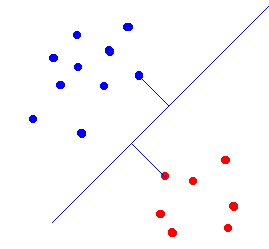
\includegraphics[width=5cm]{img/svm}
\end{center}
\caption{Наилучшая разделяющая прямая в двухмерном пространстве}
\label{svm}
\end{figure}

Если разделяющая гиперплоскость существует выборка называется \textbf{линейно разделимой}.

Для обобщения на случай линейно неразделимой выборки используется следующая идея: выборку можно сделать линейно разделимой, если увеличить размерность пространства. Для этого используется так называемая \textbf{ядерная функция}

\begin{figure}[h]
\begin{center}
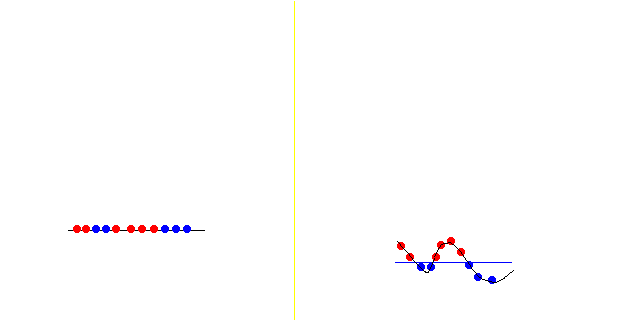
\includegraphics[width=15cm]{img/svm2}
\end{center}
\caption{Неразделимая в одномерном пространстве выборка стала разделимой после перевода в двумерное пространство}
\label{svm-kernel}
\end{figure}

Пусть признаковое пространство имеет размерность $N$, а обучающая выборка состоит из $M$ пар $(x_i, y_i)$. В таком случае обучение методом опорных векторов происходит за время, оцениваемое как
\begin{equation}
O(M^2*N)
\end{equation}
а время работы построенного классификатора $F^*(X)$ оценивается как 
\begin{equation}
O(N)
\end{equation}

Метод опорных векторов в настоящее время рассматривается как наиболее универсальный и хорошо работающий на большом количестве задач. Кроме того в работе\cite{ROZ} было показано что этот метод показывает хорошие результаты при применении его к задаче фильтрации спама. Для решения поставленной задачи мы также воспользуемся этим методом.

\subsection{Обзор существующих открытых систем фильтрации спама}
Любая система фильтрации состоит из нескольких компонентов состоит из нескольких модулей. Часть из этих модулей реализует взаимодействие с почтовым сервером, часть отвечает за выявление заголовков и тела письма, часть реализует логику фильтрации. Так как модуль, реализующий логику фильтрации, является лишь одним из нескольких необходимых модулей, имеет смысл не реализовывать систему фильтрации спама с нуля, а выбрать одну из систем с открытым исходным кодом для доработки.

Для выбора системы для доработки произведем обзор существующих открытых систем фильтрации спама в соответствии со следующими критериями:
\begin{itemize}
\item Лицензия. Лицензия должна быть открытой и позволять доработку.
\item Дата последнего релиза. Средство должно быть поддерживаемым разработчиками, и чем позднее был выпущен последний релиз, тем лучше.
\item Язык программирования. Для простоты модификации средство должно быть написано на одном широкоиспользуемых языков программирования(C, C++, Python).
\item Размещение системы фильтрации спама. Система должна размещаться на стороне сервера для того, чтобы было возможно произвести многопрофильную фильтрацию. 
\item Метод фильтрации спама - для того чтобы прозивести тестирование разработанного метода, необходимо, чтобы система использовала всего один метод фильтрации.
\end{itemize}

\textbf{spamassassin}

SpamAssassin - одно из наиболее известных открытых средств фильтрации спама. Этот проект динамично развивается и показывает хорошие результаты производительности и качества фильтрации. SpamAssassin использует в своей работе большое количество методик обнаружения спама.

\begin{itemize}
\item Лицензия: Apache License 2.0;
\item Язык программирования: Perl;
\item Дата последнего релиза: 2010г.;
\item Размещение системы фильтрации: клиент или сервер;
\item Метод фильтрации спама: большое количество различных эвристик.
\end{itemize}

\textbf{spamprobe}

Система Spamprobe написана на языке C++ и использует байесовский подход к фильтрации спама. В настоящее время практически не поддерживается, последняя версия была выпущена в 2007 году.
\begin{itemize}
\item Лицензия: Q Public License; 
\item Язык программирования: C++;
\item Дата последнего релиза: 2007г.;
\item Размещение системы фильтрации: сервер;
\item Метод фильтрации спама: байесовская классфикация.
\end{itemize}

\textbf{bogofilter}

Система работает на стороне клиента, может интегрироваться в различные почтовые клиенты(такие как kmail и evolution). Использует в своей работе байсовские методы.
\begin{itemize}
\item Лицензия: GPL v.2; 
\item Язык программирования: C;
\item Дата последнего релиза: 2010 г.;
\item Размещение системы фильтрации: почтовый клиент;
\item Метод фильтрации спама: байесовская классфикация.
\end{itemize}

\textbf{bmf}

Очень маленький по размеру (около 4000 строк кода) спам-фильтр. Использует байесовский подход к фильтрации спама. в настоящее время не поддерживается.
\begin{itemize}
\item Лицензия: GPL; 
\item Язык программирования: C;
\item Дата последнего релиза: 2002 г.;
\item Размещение системы фильтрации: сервер;
\item Метод фильтрации спама: байесовская классфикация.
\end{itemize}

\textbf{Quick Spam Filter}

Использует байесовский подход к фильтрации спама. Написан на языке C, в связи с чем работает достаточно быстро. В настоещее время не поддерживается.
\begin{itemize}
\item Лицензия: Artistic License 2.0;
\item Язык программирования: C;
\item Дата последнего релиза: 2004г.;
\item Размещение системы фильтрации: сервер;
\item Метод фильтрации спама: байесовская классфикация.
\end{itemize}

\textbf{scmail}

Написан на языке scheme. Для фильтрации использует различные эвристическии подходы. В настоящее время не поддерживается.
\begin{itemize}
\item Лицензия: BSD License;
\item Язык программирования: Scheme;
\item Дата последнего релиза: 2004г.;
\item Размещение системы фильтрации: сервер;
\item Метод фильтрации спама: различные эвристики.
\end{itemize}

\textbf{Spambayes}

Написан на языке python, поэтому достаточно прост в модификации. Работает на стороне почтового клиента.

\begin{itemize}
\item Лицензия: PSF License;
\item Язык программирования: Python;
\item Дата последнего релиза: 2011г.;
\item Размещение системы фильтрации: почтовый клиент;
\item Метод фильтрации спама: байесовская классификация.
\end{itemize}



\textbf{dspam} 

Открытая система фильтрации спама. Dspam изначально проектриовался для работы в многопользовательском режиме.
\begin{itemize}
\item Лицензия: GPL v.2;
\item Язык программирования: C;
\item Дата последнего релиза: 2011г.;
\item Размещение системы фильтрации: Сервер.
\item Метод фильтрации спама: байесовская классификация.
\end{itemize}

Для фильтрации спама dspam может использовать одну из нескольких разновидностей байесового классификатора.
Dspam написан на языке С и работает достаточно эффективно. Dspam имеет большое сообщество разработчиков и активно развивается в настоящий момент.
Из недостатков системы dspam можно отметить использование устаревшей системы сборки (autools) и использование низкоуровневой разработки, что усложняет понимание и модификацию его исходного кода.
\begin{figure}[h]
\begin{center}
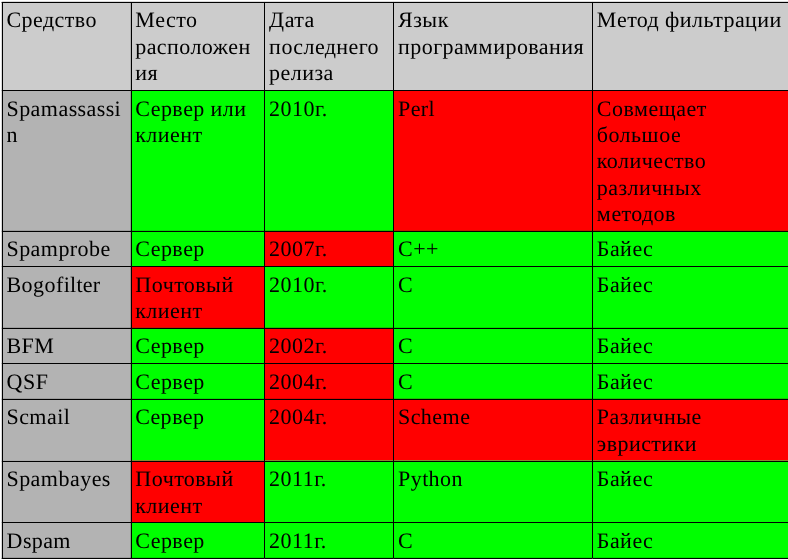
\includegraphics[width=13cm]{img/compare}
\end{center}
\caption{Сравнение систем фильтрации спама}
\label{spam_systems}
\end{figure}


Для доработки был выбран именно dspam, так как он удовлетворяет нашим требованиям, а именно:
\begin{itemize}
\item Ориентирован на работе на стороне сервера
\item Распространяется под свободной лицензией
\item Ориентирован на многопользовательский режим
\item Фильтрация спама осуществляется  всего одним алгоритмом, что упрощает тестирование разработанного метода
\end{itemize}

